
\begin{figure*}[t!]
\begin{small}
\begin{center}
\setlength\tabcolsep{4pt}
  \begin{tabular}{l | c c c c c c c c c c c c c c c c c c}
    \hline
    Query & 
    A1 & A2 & A3 & A4 & A5 & A6 & A7 & A8 & A9 & A10 & A11 & A12 & A13 & A14 &
    A15 & G1 & G2 & G3 
    \\ \hline 
    No. Of Transitions & 
    2 & 3 & 3 & 2 & 3 & 2 & 3 & 5 & 6 & 25 & 4 & 5 & 3 & 13 & 18 & 3 & 4 & 2 
    \\
    Has Union & 
     &  &  &  &  &  &  &  & $\checkmark$ & $\checkmark$ &  & $\checkmark$ &  &
     $\checkmark$ & $\checkmark$ & $\checkmark$ &  &
    \\
    Has Kleene Star & 
     &  &  &  &  &  &  &  & $\checkmark$ & 
     \begin{tabular}[c]{@{}c@{}}$\checkmark$\\(group)\end{tabular} &
     $\checkmark$ & $\checkmark$ & $\checkmark$ & $\checkmark$ & 
     \begin{tabular}[c]{@{}c@{}}$\checkmark$\\(group)\end{tabular} &  &
     $\checkmark$ &
    \\
    Has SecondaryKey & 
     & $\checkmark$ & $\checkmark$ & $\checkmark$ & $\checkmark$ &  &  & $\checkmark$ &
     $\checkmark$ & $\checkmark$ &  &  &  & $\checkmark$ &  &  &  & $\checkmark$
    \\
    Input Size(GB) & 
    216 & 321 & 477 & 264 & 1361 & 180 & 148 & 158 & 1167 & 587 & 234 & 1167 &
    286 & 366 & 141 & 593 & 593 & 85
    \\
    \hline
  \end{tabular}
\vspace{-10pt}
\end{center}
\end{small}
\caption{Workload characteristics}
\label{tab:workload}
\end{figure*}



\section{Evaluation}
\label{sec:evaluation}

We tested our approach on 2 workloads:
i) Asimov, consisting of 15 patterns (A1-15) matched over telemetry events
collected within a 2 hours interval by the Asimov system, and 
ii) GitHub, performing repository analytics (patterns G1-3) over the GitHub
dataset consisting of events collected over a 5 years period.
All transitions in a pattern have a main key constraint, i.e.\ all events in a
match should belong to the same device for the Asimov workload, or the same
repository for the GitHub patterns, and a time constraint, i.e.\ all events 
considered should occur within a timeout from the initial event in the match.
In addition, 9 patterns also have a secondary key constraint between some of
their transitions.
The characteristics of our workload are summarized in figure~\ref{tab:workload}.
The queries that we experiment with have up to 25 transitions and make use of
both {\em union} and {\em Kleene star}. 
In particular, queries A10 and A15 apply the Kleene star over a sub-pattern as
opposed to a single query variable.



We assess the benefits provided by our approach in terms of 
the ratio of input events vs selected events, 
the total execution time across the processing nodes of the cluster,
and the time it takes to complete the query (latency).
In measuring the data reduction provided by our abstract filters for a specific
query we use as baseline only the events from the input stream that satisfy the
selection predicates of some transition in the query. 
This way we can evaluate our approach in isolation from the standard technique
of pushing selection predicates into the scan operator of a query. 
The resulting amount of data to be processed by each query is detailed in
figure~\ref{tab:workload}.
Finally, we use query A5 to highlight the individual filtering potential
of different join predicates, as well as their sensitivity wrt.\ the amount of
state dedicated to their abstract representation.

\begin{figure}[t!]
\centering

\begin{subfigure}[t]{\columnwidth}
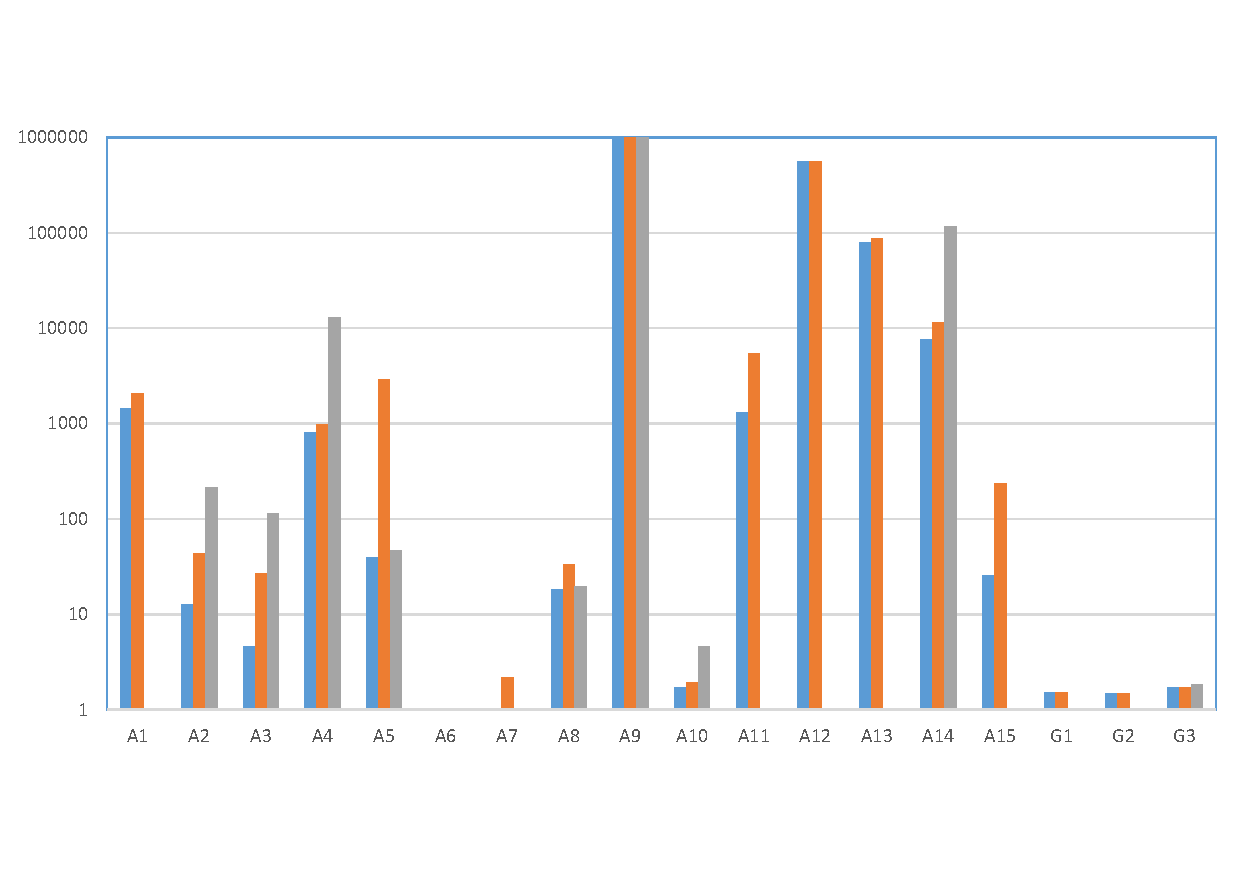
\includegraphics[clip, trim=0.3cm 1.6cm 0.4cm 1.6cm,
width=\columnwidth]{graphs/data_red.pdf}
\caption{Processed data reduction}
\label{fig:data_red}
\end{subfigure}
~
\begin{subfigure}{\columnwidth}
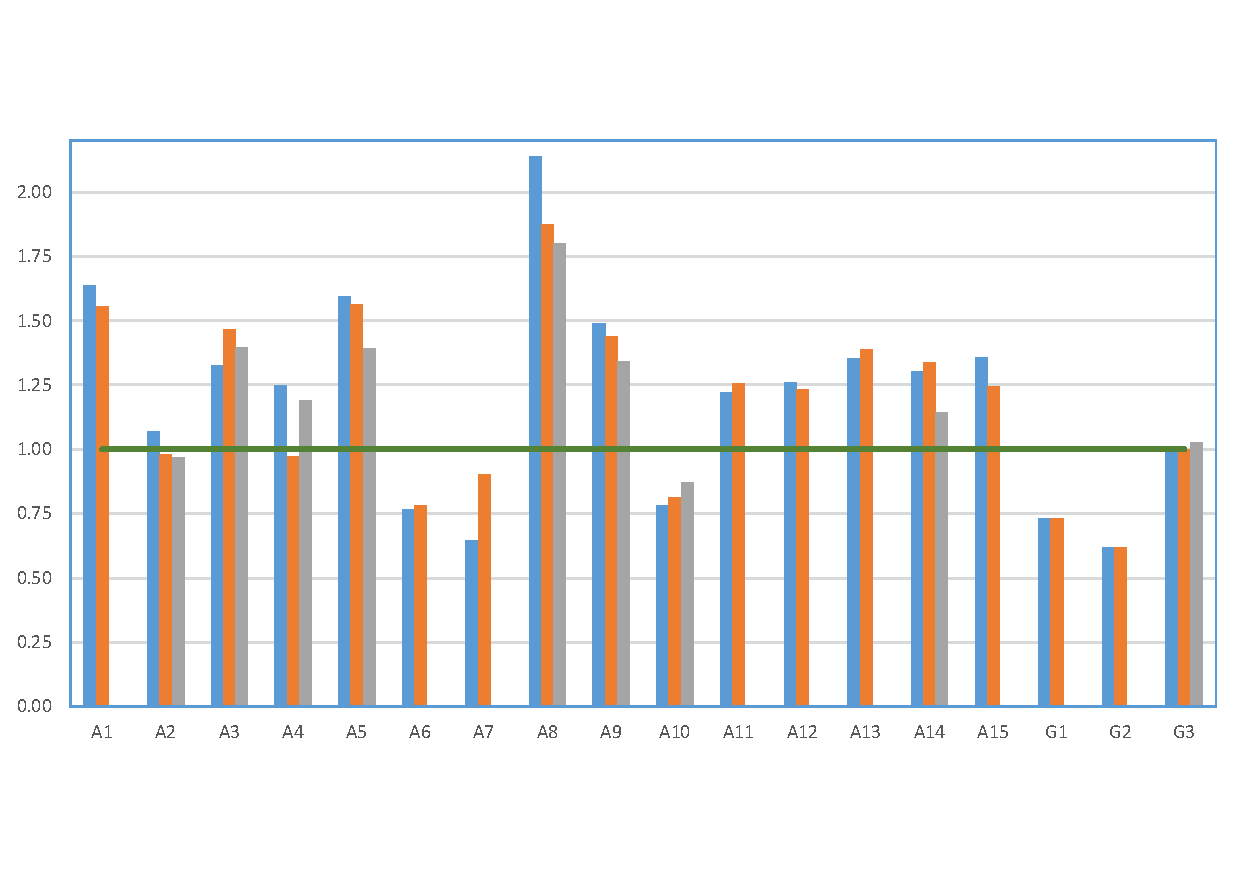
\includegraphics[clip, trim=0.3cm 2cm 0.4cm 1.8cm,
width=\columnwidth]{graphs/processing_red.pdf}
\caption{Processing time speedup}
\label{fig:processing_red}
\end{subfigure}
~
\begin{subfigure}{\columnwidth}
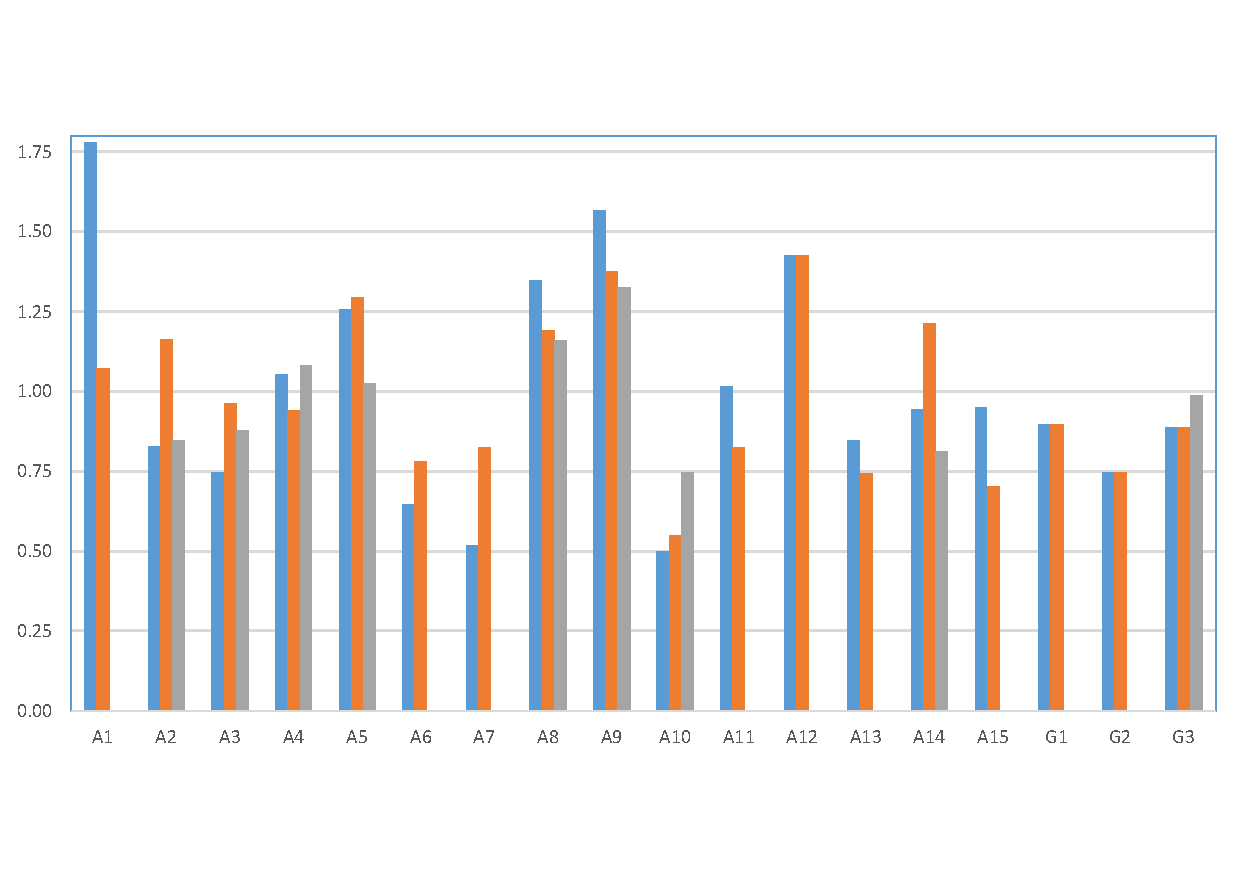
\includegraphics[clip, trim=0.3cm 2cm 0.4cm 1.8cm,
width=\columnwidth]{graphs/latency_red.pdf}
\caption{Latency speedup}
\label{fig:latency_red}
\end{subfigure}

\caption{Reduction ratios of processed data and processing speedups when using
abstract filters wrt.\ the corresponding baseline measures.}
\end{figure}


\subsection{Processed data reduction}

In order to establish the raw potential of our approach we look at the amount of
data that is discarded by the abstract filters that we build.
We note that the baseline consists only of events whose type matches the event
type of a transition in the query.

Figure~\ref{fig:data_red} shows on a logarithmic scale the ratio between the
data processed by the baseline approach and the data processed by our solution
when considering different join predicates for building the abstract filters.
In particular, we look at three types of join predicates: those referencing
the main join key of the query (MainKey), those imposing constraints on the
timestamp of matching events (Time), and those referencing a secondary join key
(SecondaryKey).
We report the results provided by the MainKey filter as well as its combination
with the Time and SecondaryKey filter (for queries with joins on a secondary
key).
 
For 12 out of the 18 queries in our workload we obtain at least a 10x reduction
in the amount of data that has to be considered by the pattern matcher, with 3
of them ending up processing 5 orders of magnitude less data.
The other 6 queries exhibit modest or no data reduction. This is mainly due to
the precision lost by our abstract filters, as well as the fact that not all
join predicates from a query can be efficiently abstracted over. 

While incorporating extra join predicates in the abstract filters leads to
further savings, it is dependent on the query and the stream of events which
additional join predicate would provide the most benefits.
In our workload we observe that adding the Time filter for queries A5 and A8 
provides the biggest improvement while for queries A2-4, A10, A14 and G1 the
SecondaryKey filter is more advantageous. 
Due to this variability one has to decide on a query by query basis which join
predicates to use and how much state to allocate for them within the abstract
filter.
For our workload we assign to the MainKey, Time and SecondaryKey filters between
16KB and 4MB, 8B and 180B, and 2B and 8B, respectively.
This allocation has been chosen under the constraint of a total size for the
abstract filter in the order of megabytes and while considering the
particularities of queries, for example, we take into account the fact that a
query with a large timeout window would not benefit from a finegrained Time
filter.





\subsection{Abstract filter size vs reduction ratio}

We vary the size of the abstract filter that we build as well as its
configuration in order to asses the impact on the reduction ratio it provides.
In particular, we experimented for query A5 with filters of sizes between 1024
to 8192KB and with a granularity for the MainKey filter between 65K to 2M
distinct values. For each abstract filter size and MainKey granularity we devote
the rest of available space to either the Time or the SecondaryKey filter.
Since the filters we build are multiplicative in their composition, the
granularity afforded to the Time and SecondaryKey filters varies between 4 and
1024 distinct values depending on the granularity of the MainKey filter as well
as the total size of the abstract filter.
In addition we record for reference the reduction in data achieved just by the
MainKey filter for its different configurations.

From the results presented in figure~\ref{fig:tradeoff} we conclude that for
query A5, MainKey+Time is the most effective configuration as it provides the
most reduction in the number of input events irrespective of the other
parameters of the abstract filter. As expected, the bigger the size of the
abstract filter the larger is the reduction rate achieved.
We also note that the distribution of state amongst the components of the
abstract filter is also important, as refining the granularity of only one of
its components while keeping the total size of the filter fixed can experience a
sweetspot beyond which the reduction rate is negatively impacted.
This is reflected in our results for the MainKey+Time configuration where the
512K granularity setting for the MainKey component outperforms the 2M setting
across all filter sizes.
The drop in the reduction rate is a consequence of the fact that the MainKey
filter reaches a plateau, beyond which increasing its granularity no longer
increases the reduction rate, while decreasing the granularity of the Time
filter is bound to decrease its filtering power.

There is also a knock-on effect between the different components of the abstract
filter, as a poor choice for the granularity of one component can inhibit the
filtering potential of the other components as well.
For example, in query A5 a too small granularity for the MainKey filter (65K
setting in figure~\ref{fig:tradeoff}) results in poor performance for the
SecondaryKey component as well, as it cannot cope with the large number of
events and their associated secondary keys it needs to discriminate between.
Notably, the Time component is less susceptible to this issue. 






\begin{figure}[tp]
	\centering
	
	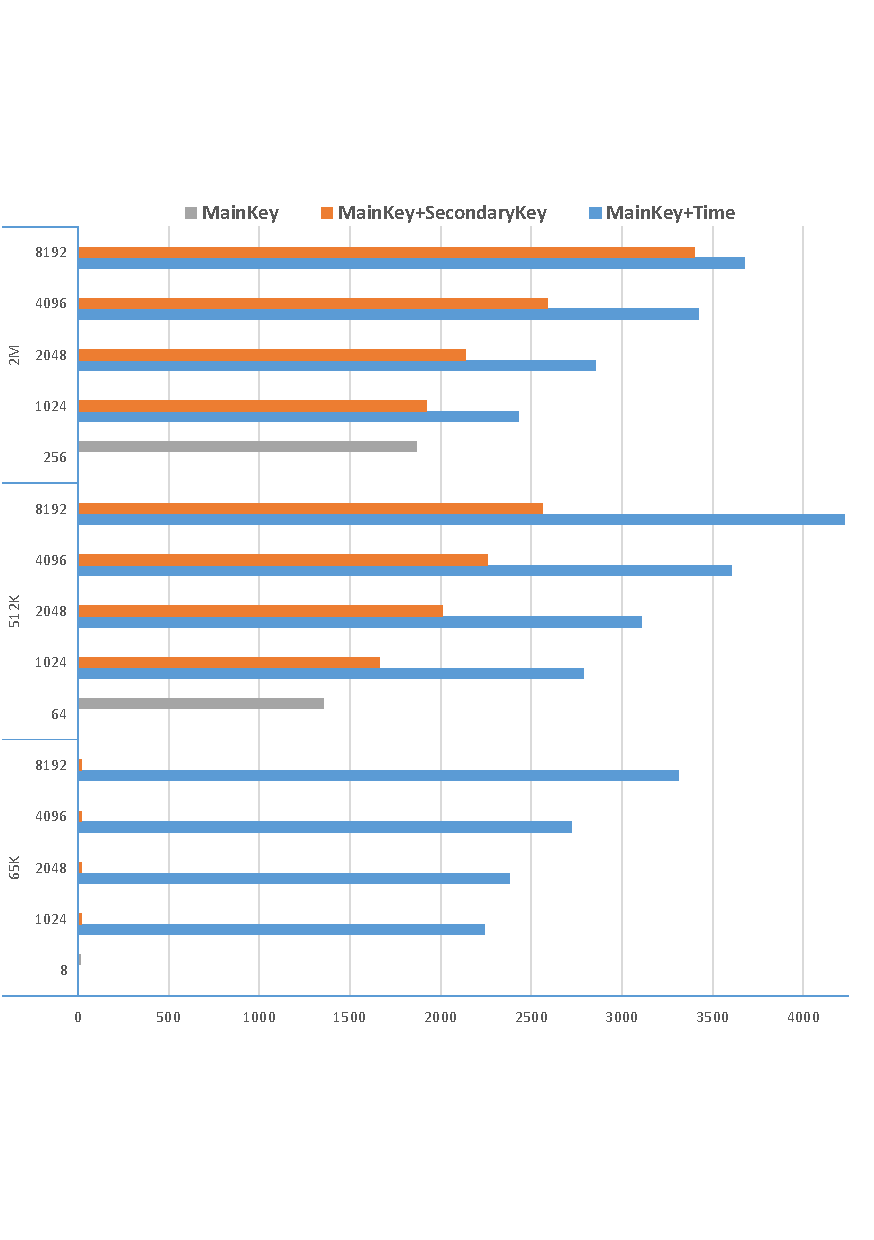
\includegraphics[clip, trim=0cm 3.5cm 0.3cm 3.7cm,
	width=\columnwidth]{graphs/A5_tradeoff.pdf}
	\caption{Tradeoff for query A5 between filter size (1024KB-8192KB) and data
		reduction for different filter configurations and with different 
		granularities
		for the MainKey filter (65K,512K,2M).}
	\label{fig:tradeoff}
\end{figure}

\subsection{Total processing time speedup}

In the following we look at the total processing cost across all nodes in the
cluster.
This is a particularly relevant metric for cluster setups that allow workload
consolidation or data centers that charge users based on total number of
``processing hours'' consumed.
Figure~\ref{fig:processing_red} shows speedups of 1.25x to 2.14x for 11 out of
the 18 queries, while 5 patterns experience slowdowns of at most 0.62x.
The slowdowns are a consequence of performing an additional pass over the input
in order to build the abstract filters, with little or no benefit in terms of
discarded events.

In order to highlight the tradeoffs of our approach we break down the {\em
baseline} execution of a query into the time it takes to 
i) read and sort the data, and 
ii) perform the reduction step.
On the other hand for our technique we look at the time it takes to 
i) read the data, 
ii) build the symbolic state associated with each transition,
iii) reduce the symbolic state associated to each transition down to an abstract
filter for the entire query and broadcast it back to every mapper,
iv) filter the input events based on the abstract filter, and
v) perform the reduction step over the remaining events. 

By discarding some of the input events our solution cuts the cost
of the sorting and reduction phases when compared to the baseline approach,
while adding the overhead of building and applying the abstract filters.
When the number of events removed is significant this leads to an overall lower
processing time as can be seen in figure~\ref{fig:breakdown}.
Since every join predicate included in the abstract filter incurs additional
costs when building and applying the filter, to maximize performance one should
consider only the smallest/cheapest set of predicates able to filter the input
down to the order of gigabytes/tens of gigabytes.


In particular we remark that the additional reduction in data provided by the
Time filter for query A5 does not translate in lower processing time (see
figure~\ref{fig:A5}).
This happens because the default MainKey filter already drastically reduces
the amount of data that needs to be processed by the pattern matcher. 
Therefore the performance gain from further reduction is easily canceled by the
cost of building the additional filter.
A similar situation occurs in query A3 where the sweet-spot is provided by the
combination of MainKey and Time predicates, even though the combination of
Main and Secondary Key filters manages to discard the largest number of events 
(figure~\ref{fig:A3}).





\begin{figure}[tp]
\centering

\begin{subfigure}[t]{\columnwidth}
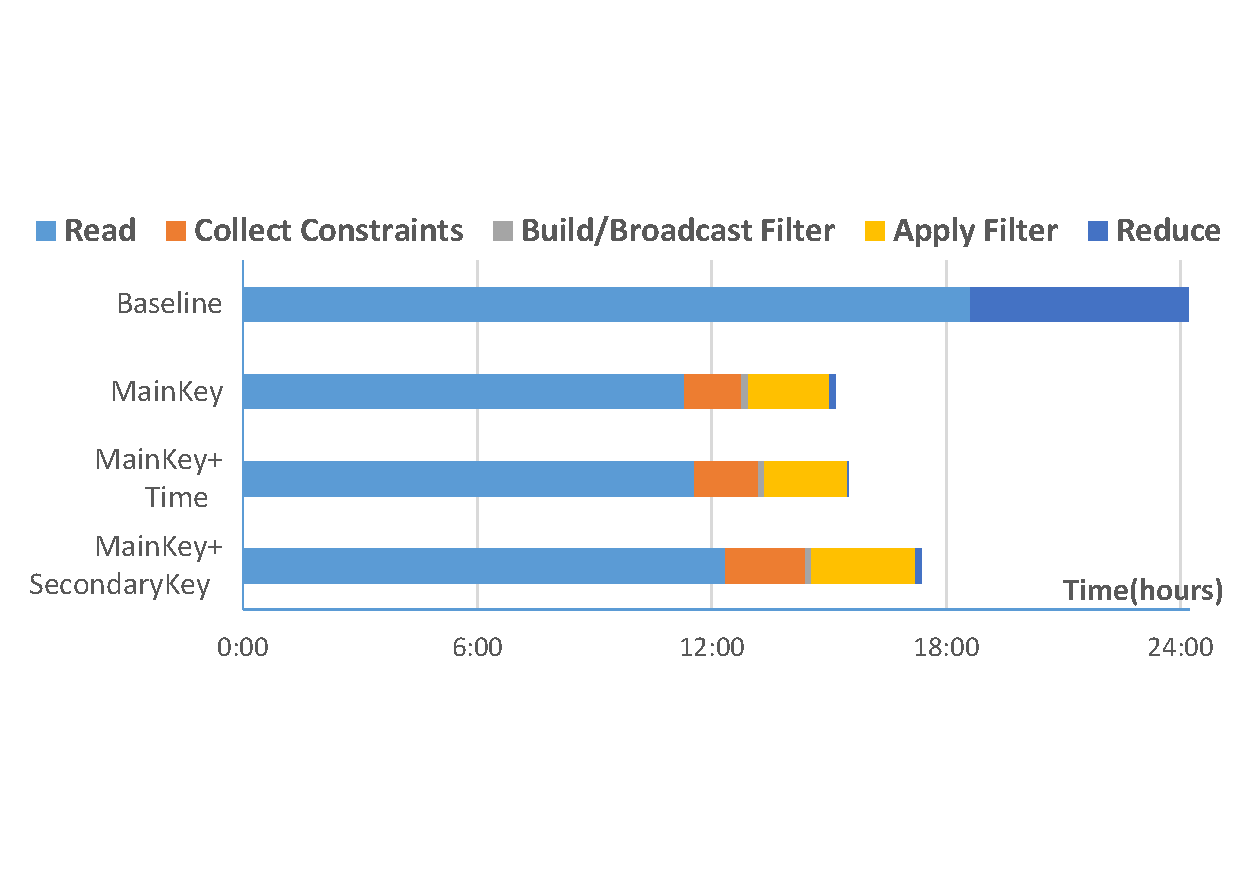
\includegraphics[clip, trim=0.5cm 3.5cm 0.9cm 3.5cm,
width=\columnwidth]{graphs/A5_breakdown.pdf}
\caption{A5}
\label{fig:A5}
\end{subfigure}
~
\begin{subfigure}[t]{\columnwidth}
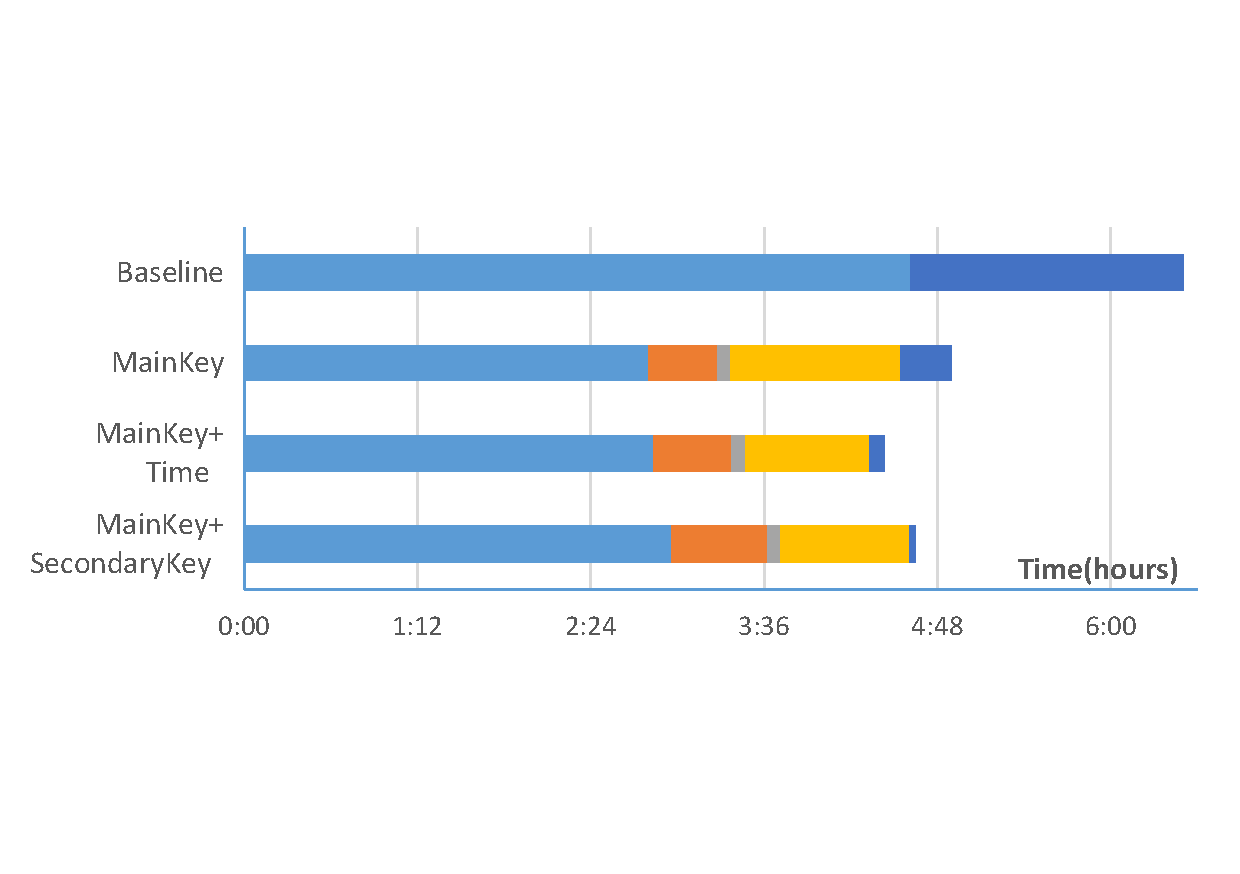
\includegraphics[clip, trim=0.5cm 4cm 0.9cm 4cm,
width=\columnwidth]{graphs/A3_breakdown.pdf}
\caption{A3}
\label{fig:A3}
\end{subfigure}

\caption{Breakdown of the total processing time for queries A5 and
A3.}
\label{fig:breakdown}
\end{figure}




\subsection{Latency speedup}


In terms of end-to-end running times we record speedups between 1.08x and 1.78x
for 8 out of the 18 queries in our workload, while for 4 of them our
approach performs within 5\% of the baseline (see Figure~\ref{fig:latency_red}).
Just like in the case of processing times, the slowdowns in latency mainly
correspond to queries for whom the abstract filters do not significantly reduce
the amount of data processed by the pattern matcher (below 5x).


We examine the performance of queries A12 and A13 as it highlights another
important factor in the latency speedup achieved by our approach.
While for both queries the abstract filters discard a significant number of the
input events and as such have smaller total processing times than the baseline,
only for A12 this translates in smaller end-to-end running times.
This happens due to the difference in the initial size of the input, 1.2TB for
A12 vs 307GB for A13, which when processed on a 85 nodes cluster results in
average running times of the reduction phase of 3.8 minutes for A12 vs 46
seconds for A13. 
Even though in our approach the reduction phase for A13 takes only 5.6 seconds
on average due to the smaller number of events being processed, that is not
enough to compensate for the additional latency introduced by the phases that
build and broadcast the abstract filters.
While the latency of these phases can be minimized by decentralizing the process
of building the abstract filters, developing and deploying such techniques falls 
outside the scope of our current work.
% same reason for A15

















